%%%%%%%%%%%%%%%%%%%%%%%%%%%%%%%%%%%%%
%% Appendix for Thesis
%% 
%%%%%%%%%%%%%%%%%%%%%%%%%%%%%%%%%%%%%

%\documentclass{agujournal2018}

%\journalname{Geophysical Research Letters}

\documentclass[main.tex]{subfiles}

\begin{document}

%% This command needs article title as argument to \supportinginfo{}:
%\supportinginfo{Antigorite Creep at Subduction Conditions: Long Duration, High Accuracy Rheological Tests On Intact Cores Using a Re-Designed Griggs Assembly}

%\authors{Eric Burdette and Greg Hirth}


%\affiliation{1}{Department of Earth, Environmental and Planetary Sciences, Brown University, Providence, RI, USA}

%\correspondingauthor{Eric Burdette}{eric\_burdette@brown.edu}

\section{Dehydrating Creep Data}\label{ch2_620}

Additional data was collected at 620°C using the same methods, materials, and assembly as other creep experiments above 400°C. This is slightly above the reaction equilibrium line between antigorite and Forsterite+Talc \citep{wunder1997antigorite}. The deviation from behavior of lower temperature samples is notable, but possibly an entirely different and not fully explored mechanism so it is addressed here separately.

\begin{figure}
  \includegraphics[width=\textwidth]{Sections/Chapter2/Figures/12-20data_1.65Plotsfits_w600.pdf}
  \caption[Antigorite creep plot including partially dehydrating data]{Antigorite creep data including partially dehydrating data.
  }
  \label{fig:CH2a_MechData_w620}
\end{figure}
\begin{figure}
  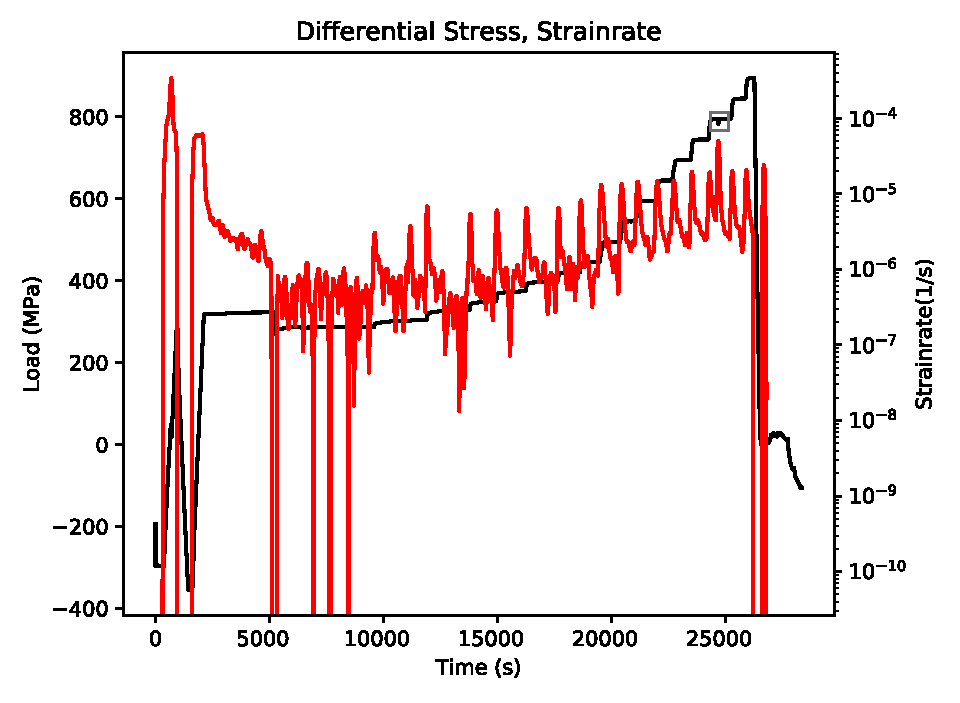
\includegraphics[width=\textwidth]{Sections/Chapter2/Figures/W2446_Stress-Strainrate-time.pdf}
  \caption[Stress/Strain rate over time of antigorite at 620°C]{Stress (black), and strain rate (red) during creep of antigorite at 620°C. Gray box highlights stick-slip event.
  }
  \label{fig:CH2a_creep620_Strainrate-Time}
\end{figure}
% \begin{figure}
%   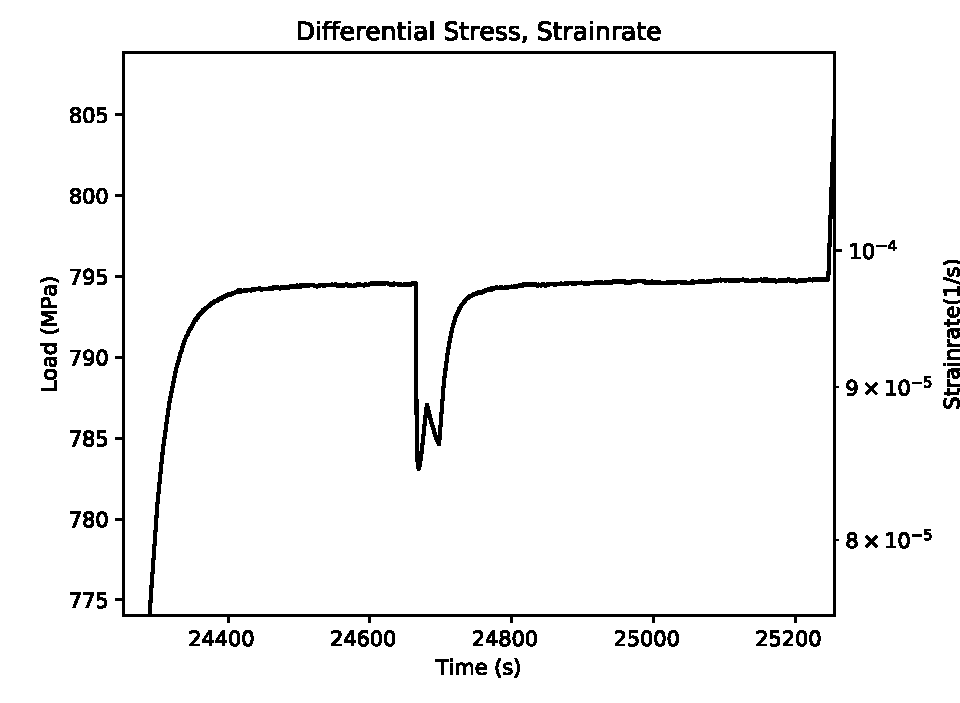
\includegraphics[width=\textwidth]{Sections/Chapter2/Figures/W2446_Stress-Strainrate-time Zoom.pdf}
%   \caption[Stick-slip event during creep at 620°C]{A zoomed in plot of stress over time showing stick slip events during antigorite creep that lead to a fault visible in recovered sections.
%   }
%   \label{fig:CH2a_creep620_Strainrate-Time_zoom}
% \end{figure}
\begin{figure}
  \includegraphics[width=\textwidth]{Sections/Chapter2/Figures/W2446_Fault_collage.pdf}
  \caption[SEM images of fault structure recovered after antigorite creep at 620°C]{a) Wide SEM image showing entire 620°C creep sample. Horizontal cracks are opened during decompression. A fault formed during deformation is visible running from the top left corner through the sample. Offset of this fault is Approximately 100 $\mu$m. b) Zoomed in view of a poorly oriented section of the fault showing grains bent nearly 120 degrees and heavily damaged. c) Zoomed in view of a smooth section of the fault. 
  }
  \label{fig:CH2a_creep620_faultCollage}
\end{figure}

Mechanical data is plotted in Figure \ref{fig:CH2a_MechData_w620} and Figure \ref{fig:CH2a_creep620_Strainrate-Time}.  Stresses of only 500 MPa are needed to deform the sample at $10^-6$ 1/s, two orders of magnitude faster than predictions of the unreacted antigorite flow law. Surprisingly, strain rate does display a systematic dependence on stress, with a power law exponent of 2.3. Strain rate evolution (hardening) is difficult to examine because experiments were completed in several hours to avoid significant reaction.

Recovered samples have less intergranular porosity and relict shear cracks than lower temperature samples, with significantly more decompression cracks. This particular sample has a single, localized fault at 35° to axial stress running one third of the length of the sample which terminates before it reaches the edge of the sample (figure \ref{fig:CH2a_creep620_faultCollage}). Approximately 100 $\mu$m offset is still visible at the top surface where the crack initiated, corresponding to the amount of stick-slip observed in mechanical data of the last loading step (Figure \ref{fig:CH2a_creep620_Strainrate-Time}. Outside of the fault there are no signs of the kinking and shear-accommodated plasticity that lower temperature samples display. The fault is generally smooth and straight, with little gouge. There are several sections in which grains were originally oriented nearly perpendicular to the fault plane. The fault is rougher in these poorly oriented sections, and grains are bent around by fault slip, tearing to form fault gouge. Several of these sections have high backscatter contrast, which could indicate reaction, but this is difficult to distinguish from edge contrast from the sharp edges of the fault and individual grains.

% Possible implications:
% \begin{enumerate}
%     \item If volume is increasing, why is strainrate so high?
%     \item Diffusional/solution flow? Would explain no plasticity
%     \item Grains rotating to form smooth fault sections?
%     \item Unstable viscosity transition with fault formation?
% \end{enumerate}


\end{document}